\begin{figure}
\centering	
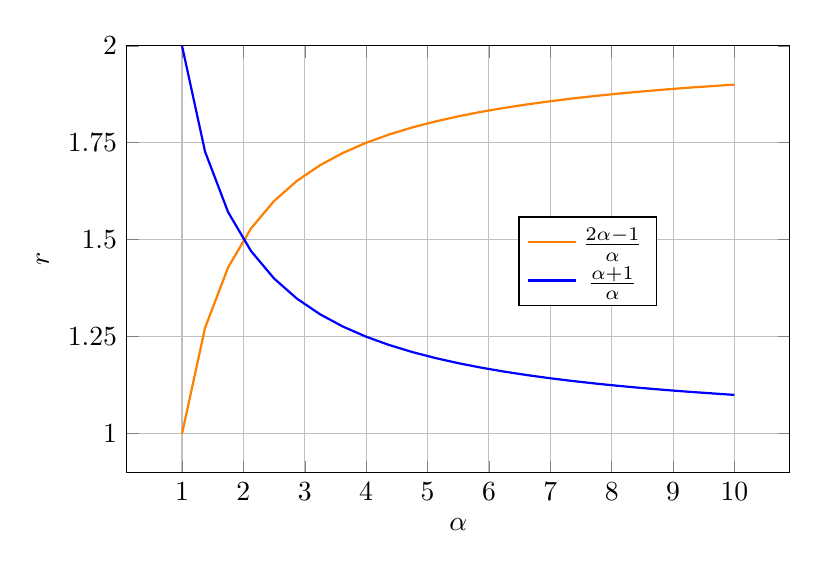
\begin{tikzpicture}
\begin{axis}[
domain=1:10, 
ymax=2,
height=7cm,
width=10cm,
xlabel = $\alpha$,
ylabel = $r$,
ytick = {1, 1.25, 1.5, 1.75, 2},
xtick = {1, 2, 3, 4, 5, 6, 7, 8, 9, 10},
grid=major,
legend style={at={(0.8, 0.6)}}
] 
\addplot[thick, orange]{(2 * x - 1) / (2 * x - x)}; 
\addplot[thick, blue]{(x + 1) / x}; 
\legend{
$\frac{2 \alpha - 1}{\alpha}$,
$\frac{\alpha + 1}{\alpha}$
}
\end{axis}
\end{tikzpicture}
\end{figure}
